\begin{figure}[t]
	\centering
	\def\u{.6em}
	\def\dist{.8}
	\def\disty{.8}
	%\tikzstyle{r}=[circle,draw=gray!80,fill=gray!20,thick,inner sep=2pt,minimum size=1.5*\u]
	\tikzstyle{r}=[circle,draw=gray!80,fill=gray!20,thick,inner sep=1pt,minimum size=1.5*\u]
	\tikzstyle{n}=[circle,draw=gray, thick,inner sep=1pt,minimum size=1.5*\u]
	\tikzstyle{arc}=[->,draw]
	\tikzstyle{edge}=[-,draw]
	%\subcaptionbox{$G(\RZ_V)$.\label{fig:test}}{
	\begin{minipage}[t]{.4\linewidth}
		\centering
		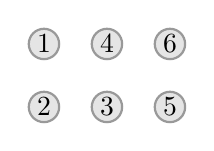
\begin{tikzpicture}
			\node[r](1) at (0,0){1};
			\node[r](2) at (0*\dist,-\disty){2};
			\node[r](3) at (1*\dist,-\disty){3};
			\node[r](4) at (1*\dist,0){4};
			\node[r](5) at (2*\dist,-\disty){5};
			\node[r](6) at (2*\dist,0){6};
		\end{tikzpicture}
		%\subcaption{}
		\subcaption{Initialization.}
		\label{fig:tree0}
	\end{minipage}
	%
	\begin{minipage}[t]{.4\linewidth}
		\centering
		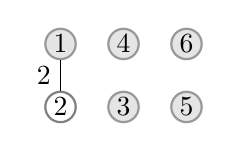
\begin{tikzpicture}
			\node[r](1) at (0,0){1};
			\node[n](2) at (0*\dist,-\disty){2};
			\node[r](3) at (1*\dist,-\disty){3};
			\node[r](4) at (1*\dist,0){4};
			\node[r](5) at (2*\dist,-\disty){5};
			\node[r](6) at (2*\dist,0){6};
			\draw(1)edge node[left]{2} (2);
		\end{tikzpicture}
		%\subcaption{}
		\subcaption{\merge{$2,1,2$}.}
		\label{fig:tree1}
	\end{minipage}

	\vspace{.5cm}
	\begin{minipage}[t]{.4\linewidth}
		\centering
		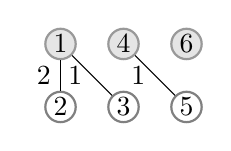
\begin{tikzpicture}
			\node[r](1) at (0,0){1};
			\node[n](2) at (0*\dist,-\disty){2};
			\node[n](3) at (1*\dist,-\disty){3};
			\node[r](4) at (1*\dist,0){4};
			\node[n](5) at (2*\dist,-\disty){5};
			\node[r](6) at (2*\dist,0){6};
			\draw(1)edge node[left]{$2$}(2);
			\draw(1)edge node[left]{$1$}(3);
			\draw(4)edge node[left]{$1$}(5);
		\end{tikzpicture}
		%\subcaption{}
		\subcaption{\merge{$3,2,1$}, then \merge{$5,4,1$}.} \label{fig:T*}
		\label{fig:tree2}
	\end{minipage}
	%
	\begin{minipage}[t]{.4\linewidth}
		\centering
		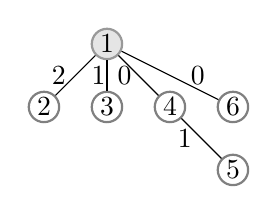
\begin{tikzpicture}
			\node[r](1) at (0,0){1};
			\node[n](2) at (-1*\dist,-\disty){2};
			\node[n](3) at (0*\dist,-\disty){3};
			\node[n](4) at (1*\dist,-\disty){4};
			\node[n](5) at (2*\dist,-2*\disty){5};
			\node[n](6) at (2*\dist,-\disty){6};
			\draw(1)edge node[left]{$2$}(2);
			\draw(1)edge node[left, xshift=3pt]{$1$}(3);
			\draw(1)edge node[left, xshift=1pt]{$0$}(4);
			\draw(1)edge node[right, xshift=4pt]{$0$}(6);
			\draw(4)edge node[left]{$1$}(5);
		\end{tikzpicture}
		%\subcaption{}
		\subcaption{\merge{$4,1,0$}, then \merge{$4,6,0$}.} \label{fig:T*}
		\label{fig:tree3}
	\end{minipage}
	\caption{
		Construction of a rooted tree that represents the hierarchical clustering solution, where a root node is
		highlighted in gray. (a) Initially, we start with an empty forest without edges where each node is a root. (b), (c), and (d) show different stages of building the tree according to
		Algorithm~\ref{algo:aic-tree}. (d) is the final tree representing the clustering solution. Now,
		for any $`g$, the clustering solution can be obtained from the tree in (d) according to Definition~\ref{def:data-structure}, i.e., by removing all
		edges of weight $\leq \gamma$ and returning the connected components as the clustering
		solution. 
		%(a) Initializaiton 
		%(b) \merge{$2,1,2$};
		%(c) \merge{$3,2,1$} \merge{$5,4,1$};
	}
	\label{fig:eg-data}
\end{figure}
